\begin{bio}

\begin{wrapfigure}{l}{0.45\textwidth}
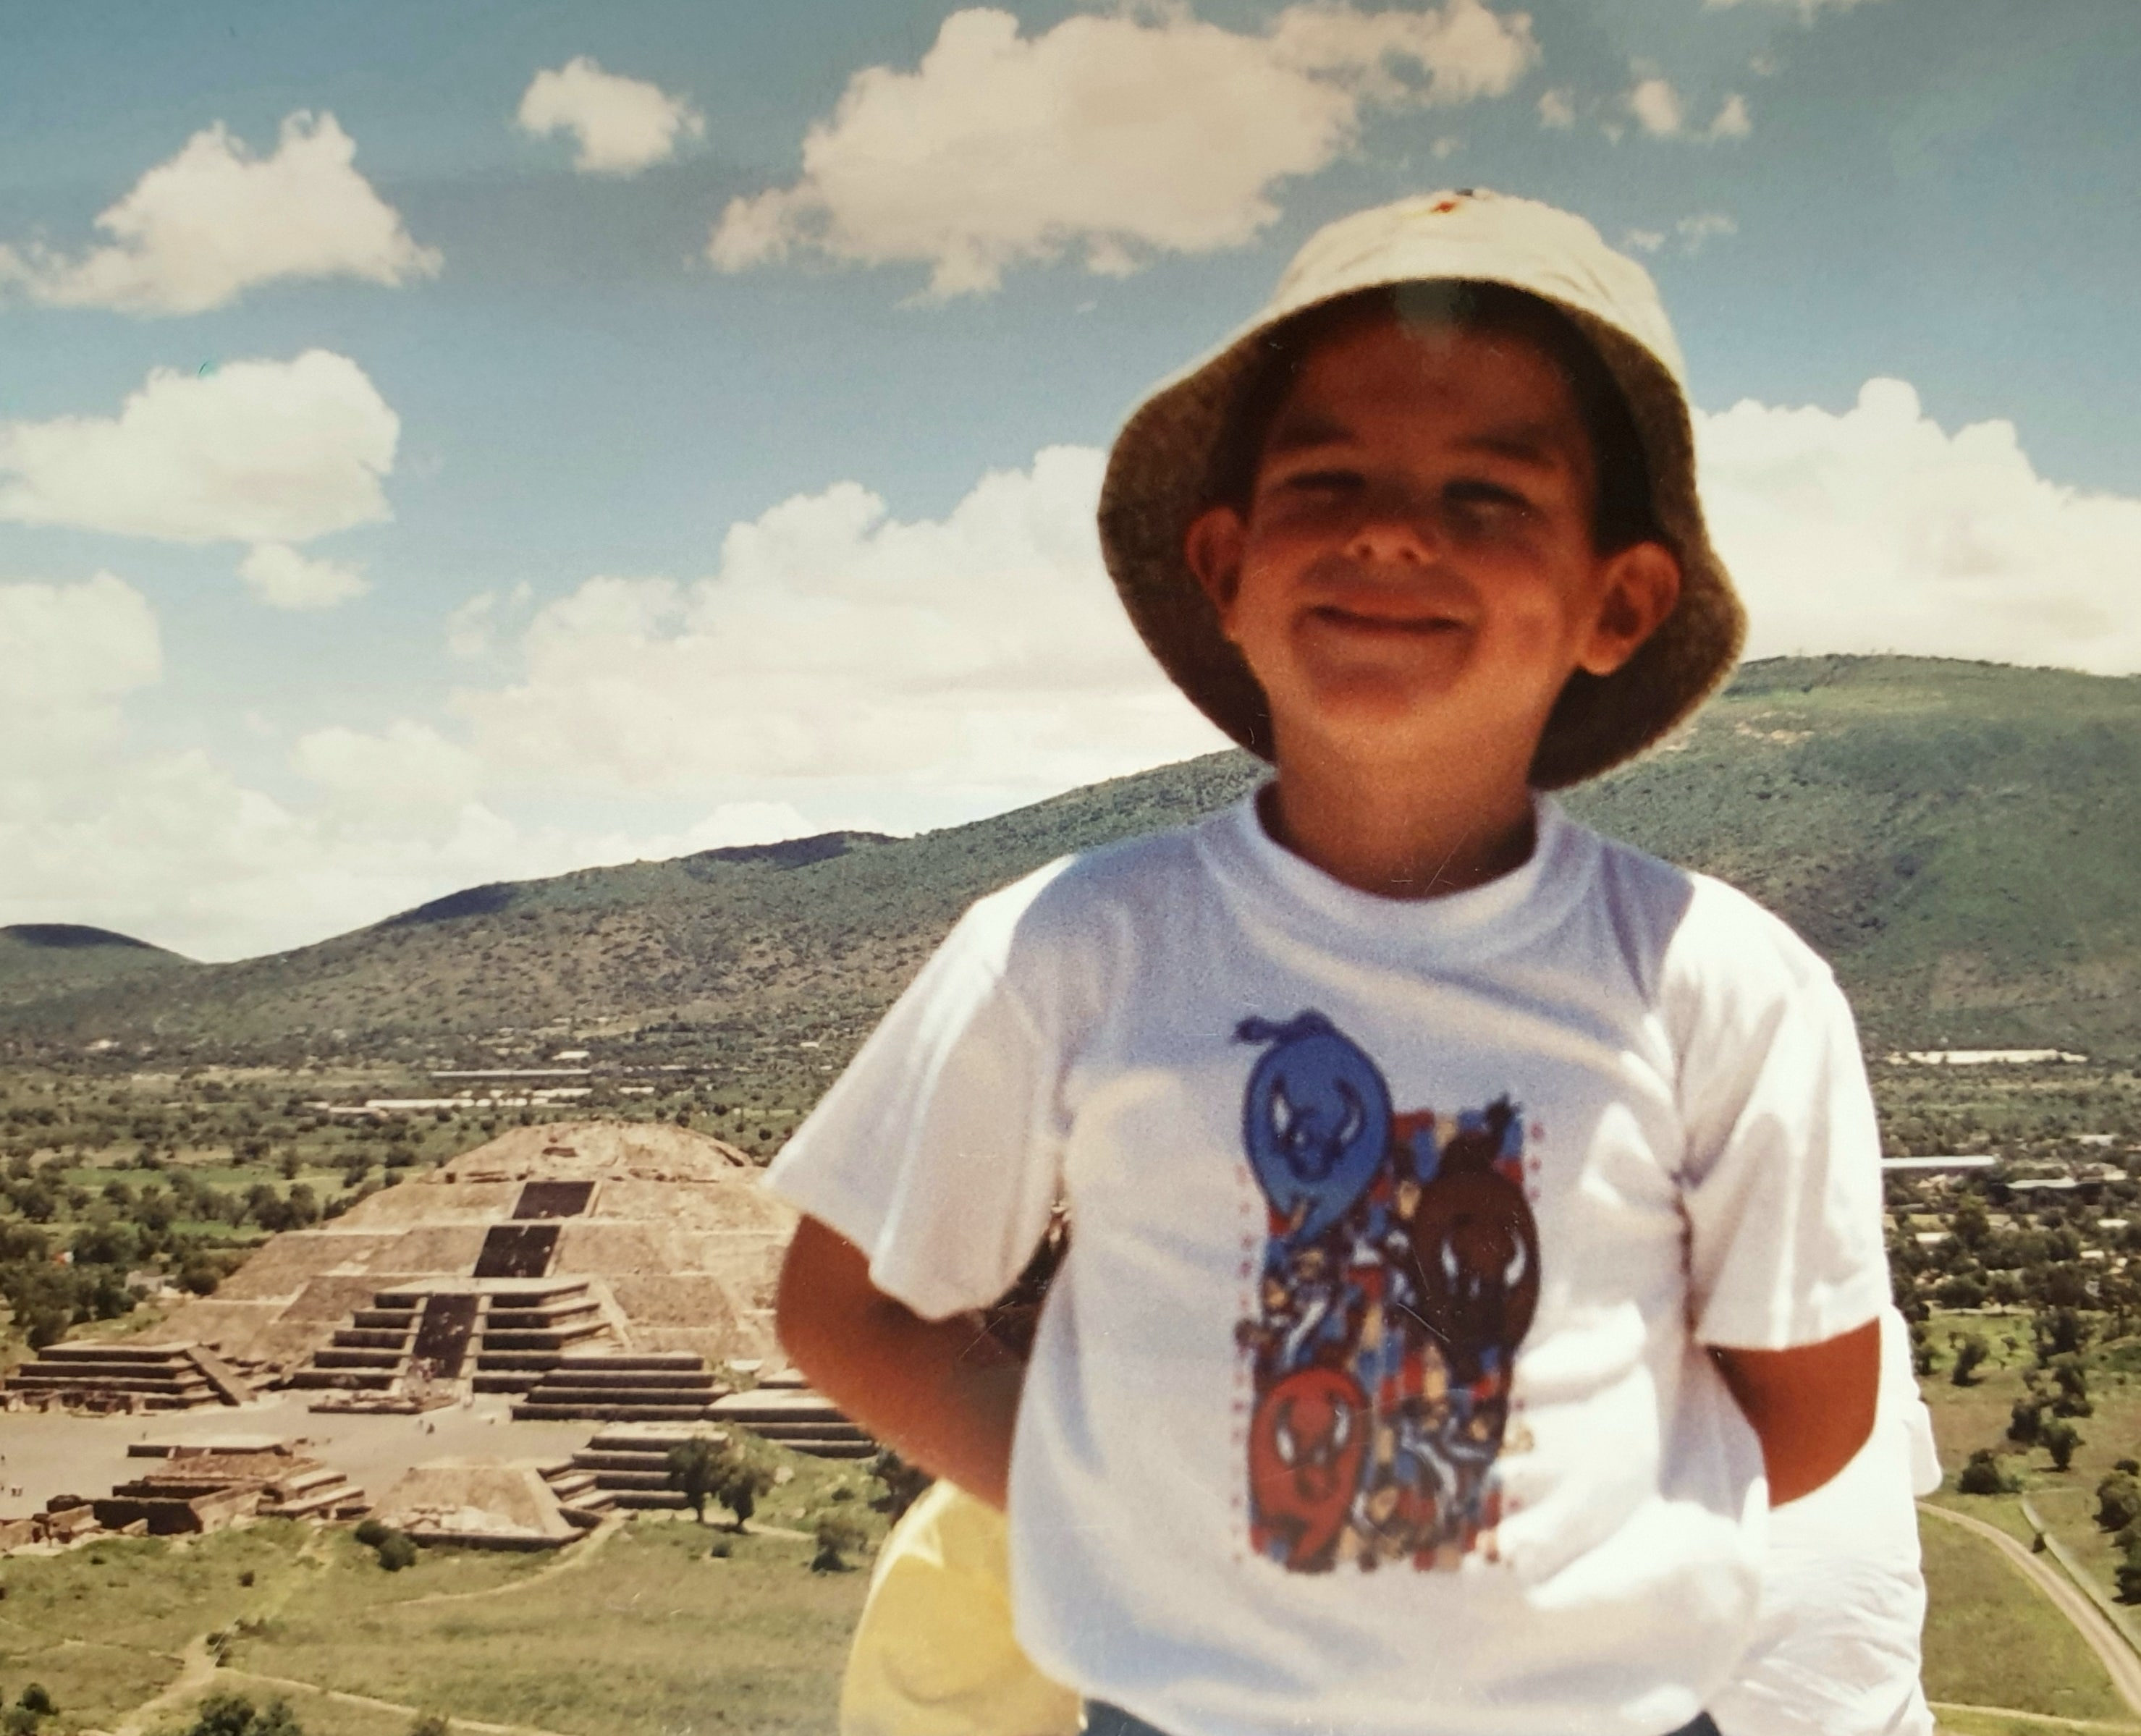
\includegraphics[width=0.96\linewidth]{header/rodri-min.jpg} 
\end{wrapfigure}
Rodrigo Castellanos García de Blas was born in Toledo, Spain, on the 22$^\text{nd}$ of February 1995. He was the first and unexpected son of a young couple. His arrival to the family did not stop his parents from being adventurous, fond of travelling and rather mad as well. From an early age, Rodrigo travelled around the globe with his parents, being strongly influenced by different cultures during his whole life. Although not very passionate about school and studying at first, he found his passion in mathematics at the age of 14. He rapidly found interest in physics, biology and even economics. Rodrigo also showed a peculiar sympathy for British culture and language, frequently visiting the UK. His devotion to science and mathematics encouraged him to study for the International Baccalaureate at the age of 16, allowing him to enrol in exchange programs in Prague and Oslo. Eventually, he decided to study for the Bachelor in Aerospace Engineering at Universidad Carlos III de Madrid in 2013, followed by the Master in Aeronautical Engineering in 2017. His interest in mathematics and fundamental physics pushed him towards research life, collaborating with the professor of aeroelasticity and aircraft design in the study of an unconventional aircraft design, the Prandtl plane. In his path at university, he also collaborated in the formula student team as aerodynamics and head of the marketing department. His enterprising nature almost pull him away from his research career but he was captivated by the thesis proposal in experimental aerodynamics by Prof. Discetti and Prof. Ianiro. In 2019, he began his PhD in the experimental aerodynamics and propulsion group at the same university, a venture that ended in late 2022. Rodrigo became an extremely self-demanding person both in his professional and personal life, ceaselessly seeking the best opportunities. In his scarce free time, Rodrigo enjoys music, gastronomy, motorsports and scuba diving. Nonetheless, his ultimate joy is travelling and discovering new cultures and friends.
\end{bio}